%!TEX root = ../MainBody.tex

% 第三章
\chapter{系统设计}% 使用\cite{}命令引用数据库中文献
\section{相关概念}
\subsection{TypeScript}
TypeScript是一种由微软开发的自由和开源的编程语言。它是JavaScript的一个严格超集,并添加了可选的静态类型和基于类的面向对象编程的首席架构师以及Delphi和Turbo Pascal的创始人安德斯·海尔斯伯格参与了TypeScript的开发。TypeScript支持为现存JavaScript库添加类型信息的定义文件,方便其他程序像使用静态类型的值一样使用现有库中的值。当前有第三方提供常用库如MongoDB、Node.js和D3.js等的定义文件。TypeScript是一种给JavaScript添加特性的语言扩展。增加的功能包括:类型批注和编译时类型检查、类型推断、类型擦除、接口、枚举、泛型编程、Mixin、命名空间、元组、await等。运行于任何平台上的任何网页浏览器都可以运行TypeScript:由于它仅仅是被编译为标准的JavaScript,一个脚本不仅可以被预编译为文件,也能通过为TypeScript包含JavaScript编译器进行实时编译。
\subsection{React}
React是一个高效而且灵活的用来构建用户界面的框架。具有声明式、组件化的特点。React视图通常采用包含以自定义HTML标记规定的其他组件的组件渲染。React为程序员提供了一种子组件不能直接影响父组件("data flows down")的模型,数据改变时对HTML文档的有效更新,和现代单页应用中组件之间干净的分离。

它由Facebook、Instagram和一个由个人开发者和企业组成的社群维护。根据JavaScript分析服务Libscore,React当前正在被Netflix、Imgur、Bleacher Report、Feedly、Airbnb、SeatGeek、HelloSign等很多网站的主页使用。
\subsection{Webpack}
Webpack 是一个成熟的开源前端模块化打包工具。Webpack 提供了前端开发缺乏的模块化开发方式,将各种静态资源视为模块,并从它生成优化过的代码

Webpack可以从客户端、或是更改 webpack.config.js配置文件来设置各项功能。

本质上,*webpack* 是一个现代 JavaScript 应用程序的*静态模块打包器(module bundler)*。当 webpack 处理应用程序时,它会递归地构建一个*依赖关系图(dependency graph)*,其中包含应用程序需要的每个模块,然后将所有这些模块打包成一个或多个 *bundle*。

要使用 Webpack 前须先安装 Node.js。Webpack 其中一个特性是使用加载器(loader)来将不同类型资源转化成对应模块。开发者可以自定义加载器的顺序、格式来因应项目的需求。
\subsection{MongoDB}
MongoDB是一种面向文档的数据库管理系统,由C++撰写而成,提供高性能,高可用性和自动扩展。MongoDB中的一条记录就是一个文档,是一个数据结构,由字段和值对组成。MongoDB文档与JSON对象类似。字段的值有可能包括其它文档、数组以及文档数组。MongoDB提供高性能的数据持久化,支持丰富的查询语言,具有高可用性和水平扩展能力且支持多存储引擎。
\section{功能设计}
\subsection{读者功能模块}
\begin{itemize}
    \item 读者登录模块。用户第一次访问系统时进入的模块,读者的账号密码输入成功之后,才能进入主界面,即浏览借阅模块。
    \item 浏览借阅模块。功能点为展示图书基本信息、可借数量和提供预约借书操作,该模块展示一个馆藏图书列表,每一个列表项用卡片表示,卡片中包含书籍的基本信息、馆藏状态、是否可借等信息,并且有一个预约按钮,当书籍为可借数量大于1时,按钮可点击。
    \item 在借图书模块。该模块功能点包括展示预约图书列表和待还图书列表。预约图书列表的每一项展示预约书籍的基本信息,且有一个取消借阅按钮,点击可取消借阅。待还图书列表的每一项展示该书籍的基本信息和实际借阅日期,且有一个还书按钮,点击该按钮可提交还书申请,弹出确认框,填写物流单号,点击确认框的"确认"按钮提交还书申请。
    \item 个人信息模块。该模块的功能点为展示读者账号信息,物流地址增删改,展示收藏列表等。
\end{itemize}
\begin{figure}[H] %H为当前位置,!htb为忽略美学标准,htbp为浮动图形
    \centering %图片居中
    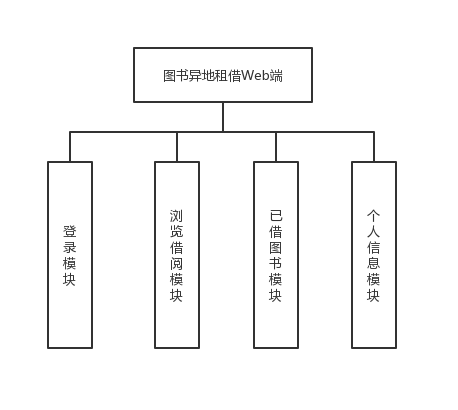
\includegraphics[width=0.7\textwidth]{./Chapters/images/reader_module.png} %插入图片,[]中设置图片大小,{}中是图片文件名
    \caption{读者模块} %最终文档中希望显示的图片标题
    \label{读者模块} %用于文内引用的标签
\end{figure}

\subsection{管理员功能模块}
\begin{itemize}
   \item 登录模块:管理员访问系统时进入的模块,系统验证成功之后,方可进入主界面。
   \item  预约列表模块:该模块功能点为展示读者预约的图书列表和预约状态修改,列表每一项包含图书名称、借书条码号、是否已借出的按钮。在管理员将书籍交付物流之后,点击该书籍所在项的按钮,弹出确认框,管理员在确认框中填写物流单号,点击确认提交信息。
   \item 待还列表模块:该模块功能点为展示通过本系统借阅的书籍、发出还书请求,但还在物流配送途中,并未被图书馆签收的书籍列表。每一项包含书籍的基本信息、借书条码号、应还日期等信息。
   \item 异常书籍模块:功能点为展示借阅过程中出现异常的书籍列表,如遗失、损坏的书籍和修改书籍异常状态。列表每一行展示异常书籍的基本信息、异常类别和异常状态修改按钮,点击该按钮可将异常书籍标记为正常,下次访问该模块时,上次标记为正常的书籍将不会展示在该模块的列表中。   
\end{itemize}

\begin{figure}[H]
    \centering
    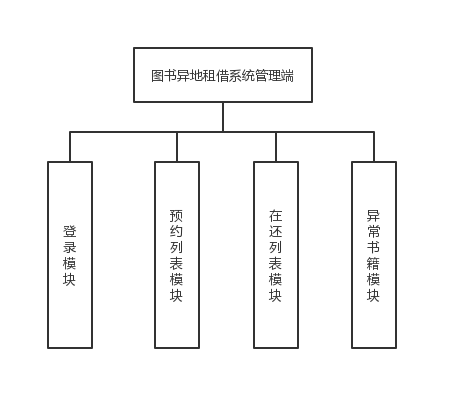
\includegraphics[width=0.7\textwidth]{./Chapters/images/admin_module.png} %插入图片,[]中设置图片大小,{}中是图片文件名
    \caption{管理员模块} %最终文档中希望显示的图片标题
    \label{管理员模块} %用于文内引用的标签   
\end{figure}
\section{架构设计}
\begin{figure}[H]
    \centering
    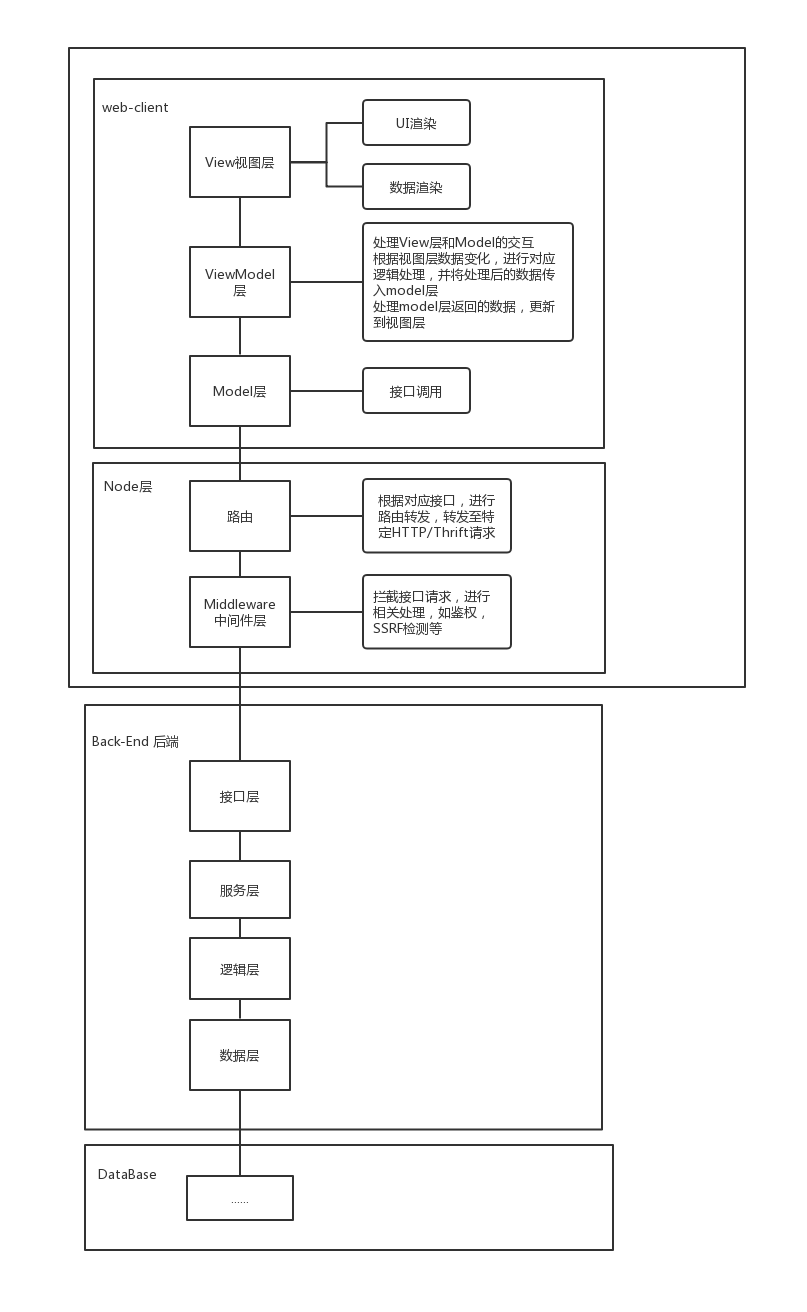
\includegraphics[width=0.7\textwidth]{./Chapters/images/system_structure.png} %插入图片,[]中设置图片大小,{}中是图片文件名
    \caption{系统架构图} %最终文档中希望显示的图片标题
    \label{系统架构图} %用于文内引用的标签   
\end{figure}
\subsection{web客户端}
web客户端采用由MVC(Model-View-Controller)架构衍生而来的MVVM架构。作为十分常见的前端架构之一,在项目中具有非常广泛的应用。MVVM架构由View层(视图层)、ViewModel层(视图模型层)、Model层(模型层)三部分组成。

视图层,是屏幕展示视图的封装,是程序中处理数据展示的部分,用于可视化界面的展示和捕捉用户进行的各种交互操作。视图层不涉及业务逻辑,只是通过访问它所监视的视图模型,实现相应视图的更新。

视图模型层,用于处理所有和业务逻辑相关的代码,完全不涉及UI部分。当View层数据发生变化时,省去中间冗余的接口,而直接驱动UI的对应变化。视图模型层承载的内容为视图展现逻辑,视图层所需的数据由视图模型层进行逻辑转换得到,转换前的初始数据可能由服务器返回、数据库获取或用户输入,这种"未经格式化"的原始数据往往无法用于视图层直接展示,视图展现逻辑就是将这些原始数据经过一系列逻辑拆分转化,处理成可以用于屏幕展示的数据。视图模型层中的每个的方法代码所处理的功能具有单一性,且与外部不产生联系,使得代码更为健壮,易于维护。

模型层。实现对业务功能和应用状态的封装,可以将其理解为同时包含数据和行为的领域模型,通常情况下模型对象负责在数据库中获取、修改数据。模型起到定义若干模板额作用,不参与实际的业务逻辑,只是对模型层进行了一层抽象,将服务端返回的JSON对象中的字段一一 映射到事先定义好的数据模型中。在业务实现中,在Model层发起具体的HTTP请求,请求经过Node层拦截处理,返回响应数据。模型层的作用实际上是实现服务端数据在web客户端的映射,这个映射过程就是web端底层发起网络请求,并获取到数据的过程,映射的结果是一个单纯的数据结构,可以用struct表征。

MVVM的核心思想是“数据模型数据为绑定”,数据绑定的关键在于视图层和视图模型层之间的信息传递,层与层之间需要进行通信交流。在MVVM架构中,这一问题是通过"观察者模式"的具体应用——响应式编程实现的。

如何实现所谓的响应式编程?在WPF中官方提供了Data Binding技术,mac系统中也有类似的Cocoa Binding框架,GitHub上也出现了RAC(ReactiveCococa)和RxSwift等第三方开源框架。
在RAC的思维中,视图层的一切均为在变化的数据流,比如用户在输入框上不断输入的文字、被点击的按钮、旋转缩放的视图等等,这些就像是一个“水龙头”,当变化产生的时候,水龙头就会出水,向下传递变化,对这个变化感兴趣的人,即订阅者(subscriber),就可以在这个水龙头上套一个"水管"。通过提供统一的消息传递机制,位于下游的接收者能够及时收到变化,拿到这个变化的具体信息,并进行相关处理。具体来说,视图层哥视图模型层互为订阅者和传播者,双向绑定数据变化,视图层更新视图,视图模型层更新数据,并将更新的数据下发至模型层。
\subsection{Node层}
为了更好的实现前后端分离,在项目中引入node作为中间层,降低耦合度,处理大量重复逻辑。node层的主要作用是作为中间层,拦截和处理网络请求,并对请求头或响应数据进行业务处理。如在request请求头中加入设置允许跨域、加入校验token等,重定向后端返回的特殊响应code、SSRF、CSRF等安全拦截、通过映射解决前后端字段参数或字段类型不统一、日志上报等。对于web客户端来说,在浏览器上做运算、做分组、以及一系列操作是一定会影响性能的、尤其数据量很大的情况,可能出现首屏加载时间长、响应速度变慢以及页面卡顿等问题,用户体验因此大打折扣。对于开发人员来说,需要处理大量本可复用的逻辑,增加代码量和开发时长,同时项目质量却下降。而使用node中间层,则相当于把众多影响性能的代码放入其中,不影响浏览器的性能,同时替后端分担一些简单的数据逻辑、处理网络请求维度的公共逻辑,使得前后端的分离更为明确和彻底。

本项目中主要使用Koa框架来实现node中间层,主要作用为转发网络请求的数据,串接前后端;路由转发,修改请求头、简单处理相应数据;处理网络请求的特殊code,根据实现约定好的code规则进行逻辑映射;拦截SSRF/CSRF等前端安全攻击;用户和不同网络请求的权限控制;日志上报等。
\begin{figure}[H]
    \centering
    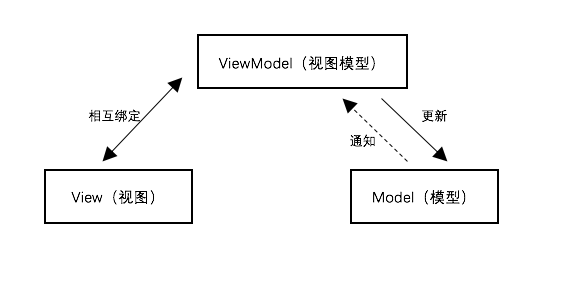
\includegraphics[width=0.7\textwidth]{./Chapters/images/mvvm.png} %插入图片,[]中设置图片大小,{}中是图片文件名
    \caption{MVVM模型} %最终文档中希望显示的图片标题
    \label{MVVM模型} %用于文内引用的标签   
\end{figure}
\section{时序图}
\begin{figure}[H]
    \centering
    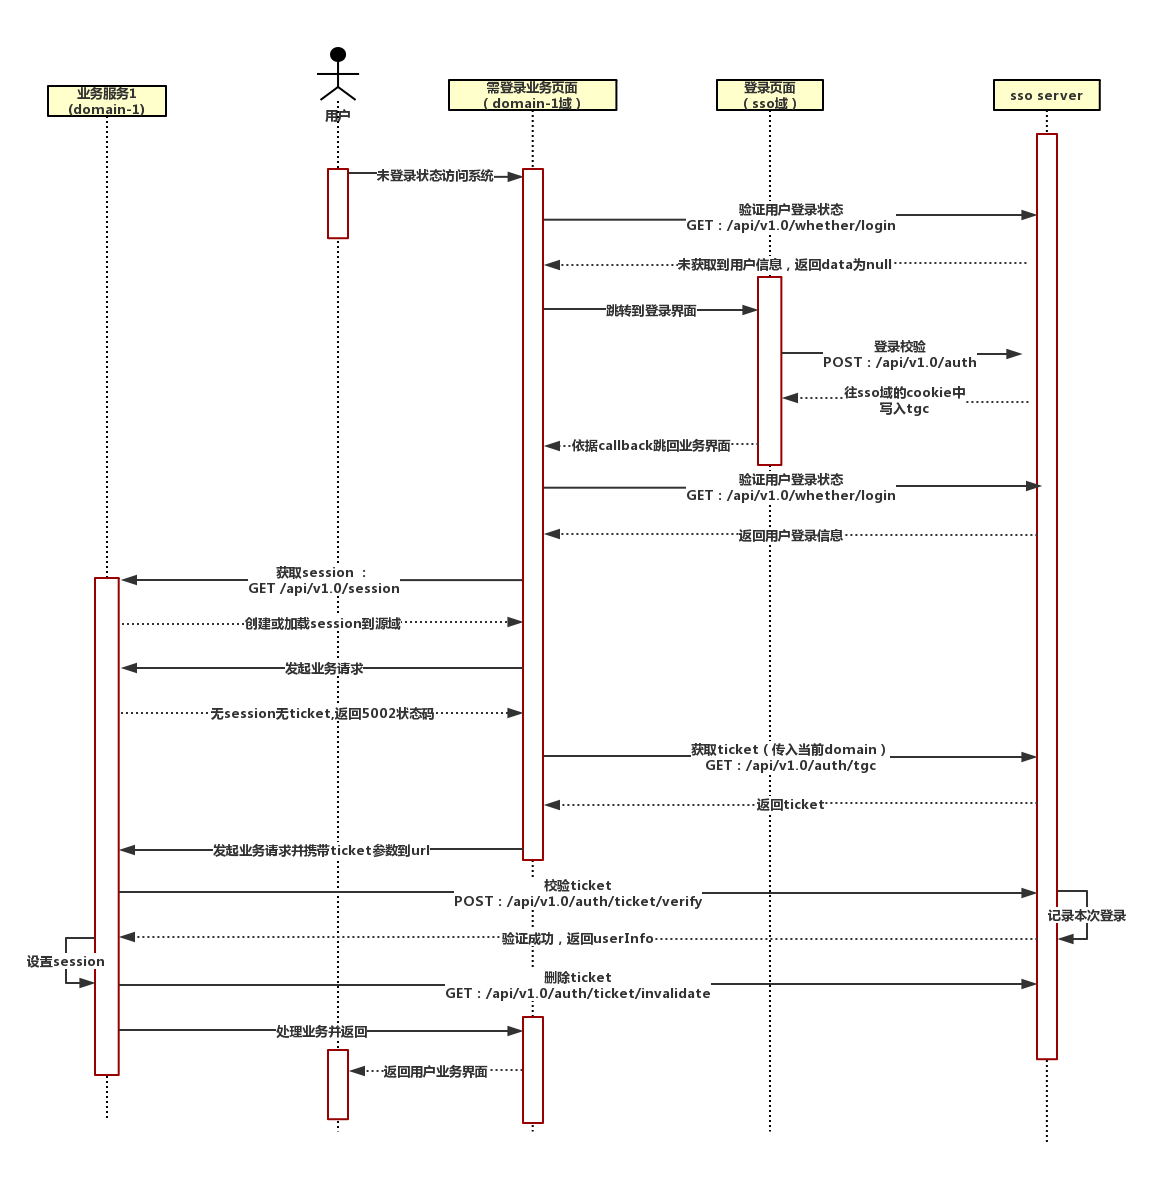
\includegraphics[width=0.7\textwidth]{./Chapters/images/time_gram_login.png} %插入图片,[]中设置图片大小,{}中是图片文件名
    \caption{登录时序图} %最终文档中希望显示的图片标题
    \label{登录时序图} %用于文内引用的标签   
\end{figure}
\begin{figure}[H]
    \centering
    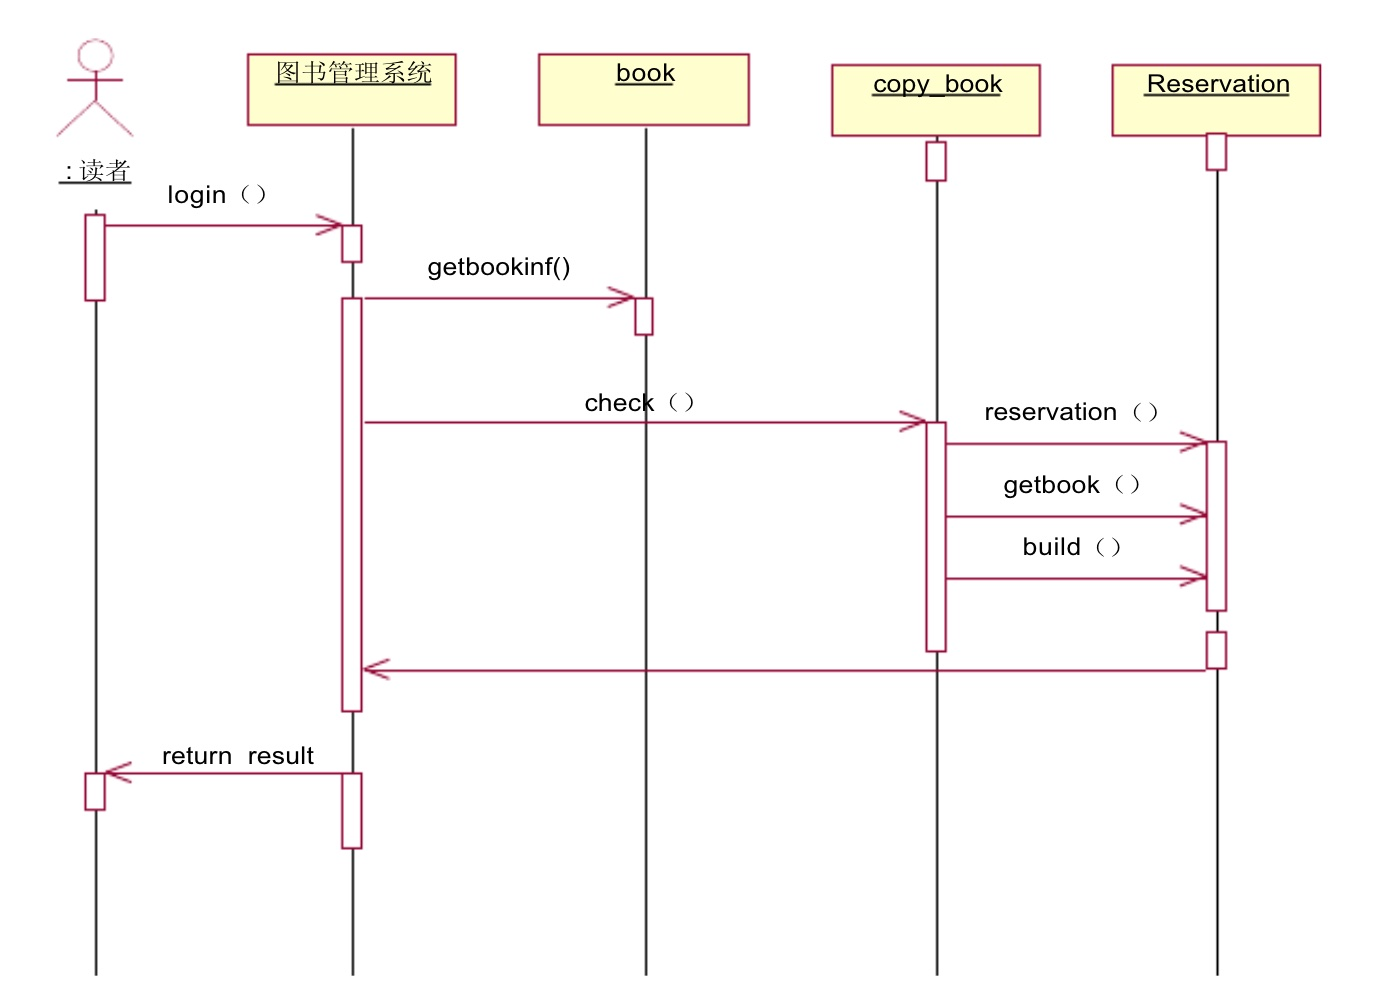
\includegraphics[width=0.7\textwidth]{./Chapters/images/time_diagram_borrow.png} %插入图片,[]中设置图片大小,{}中是图片文件名
    \caption{借书时序图} %最终文档中希望显示的图片标题
    \label{借书时序图} %用于文内引用的标签   
\end{figure}
\begin{figure}[H]
    \centering
    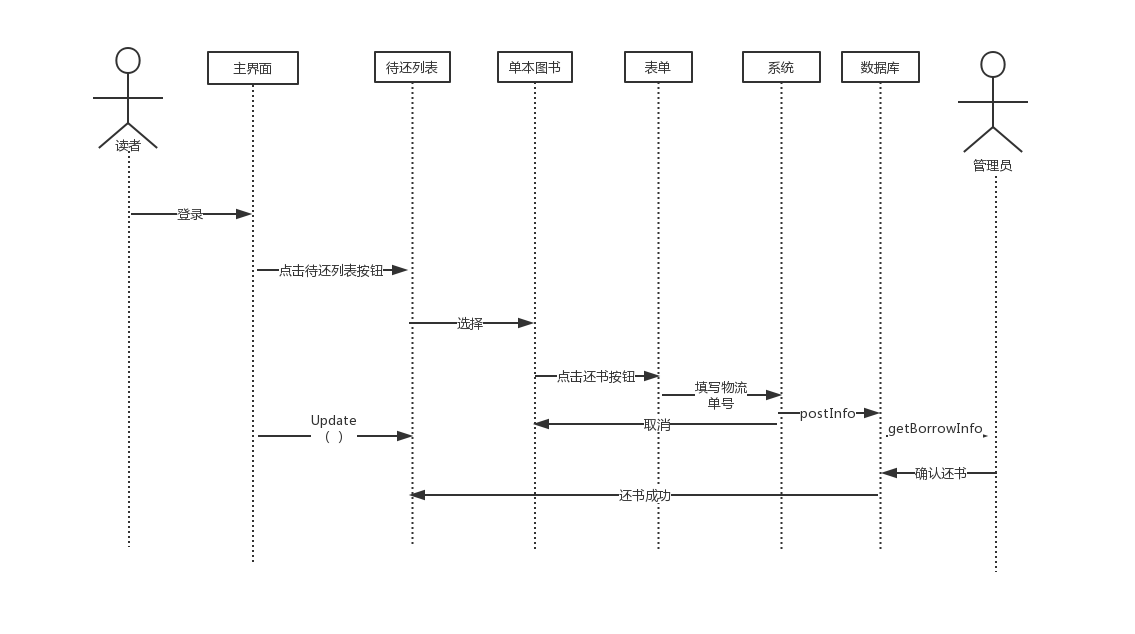
\includegraphics[width=0.7\textwidth]{./Chapters/images/time_diagram_back.png} %插入图片,[]中设置图片大小,{}中是图片文件名
    \caption{还书时序图} %最终文档中希望显示的图片标题
    \label{还书时序图} %用于文内引用的标签   
\end{figure}
\section{类图}
\begin{itemize}
    \item Reader类是读者类,包含若干属性和操作。属性有读者ID(userId)、姓名(userName)、地址(address[])、预约书目(borrowed[])、待还书目(toReturned[]),主要操作有预约借书(borrowBook)、还书(returnBook)等
    \item Admin是管理员类,包含管理员编号(adminId)、管理员姓名(adminName),操作主要有处理借书单据(handleBookBorrow)和处理还书单据(handleBookReturn)等。
    \item BookInfo是记录图书信息的类,属性包括书籍ISBN号、书籍名称、作者、出版社、内容简介等
    \item BookBorrowInfo是书籍借阅信息类,包含书籍条码号、可借数量、馆藏数量、馆藏位置等属性。
    \item Borrow是具体某书的借阅信息,包括书籍条码号、借书物流单号、还书物流单号、借阅时间等属性。
\end{itemize}
\begin{figure}[H]
    \centering
    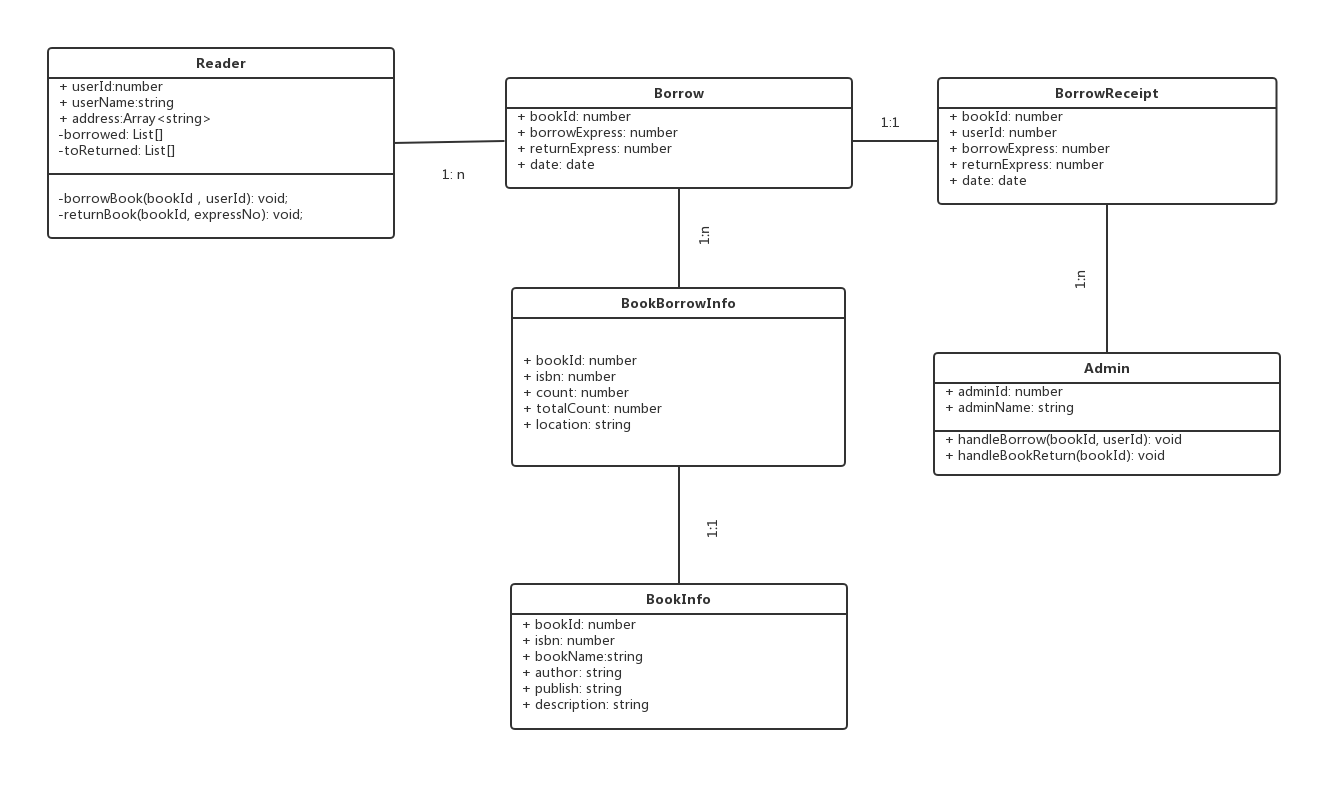
\includegraphics[width=0.7\textwidth]{./Chapters/images/class_diagram.png} %插入图片,[]中设置图片大小,{}中是图片文件名
    \caption{类图} %最终文档中希望显示的图片标题
    \label{类图} %用于文内引用的标签   
\end{figure}
% \section{数据库设计}
% \subsection{实体图}
% 读者:读者属性有账号、姓名、密码、地址、已借书籍信息、预约书籍信息。实体图如图所示:
% 图书:图书属性有图书编号、书名、作者、出版者、出版信息、总数量、可借数量、内容摘要。实体图如图所示:
% \begin{figure}[H]
%     \centering  %图片全局居中
%     \subfigure[读者实体图]{
%     \label{读者实体图}
%     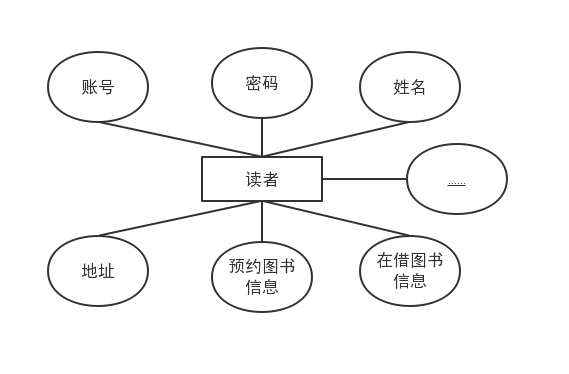
\includegraphics[width=0.45\textwidth]{./Chapters/images/reader_entity.png}}
%     \subfigure[图书实体图]{
%     \label{图书实体图}
%     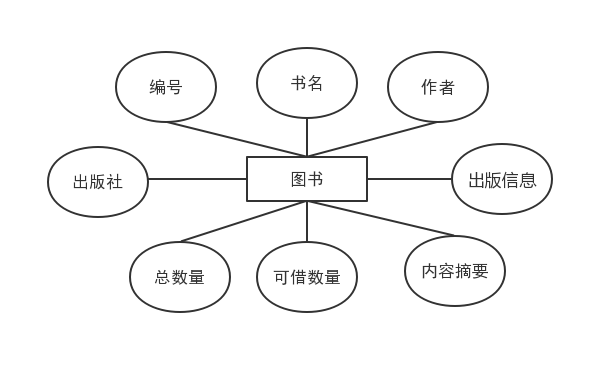
\includegraphics[width=0.45\textwidth]{./Chapters/images/book_entity.png}}
%     \caption{实体图}
%     \label{实体图}
% \end{figure}
% \begin{figure}[H]
%     \centering
%     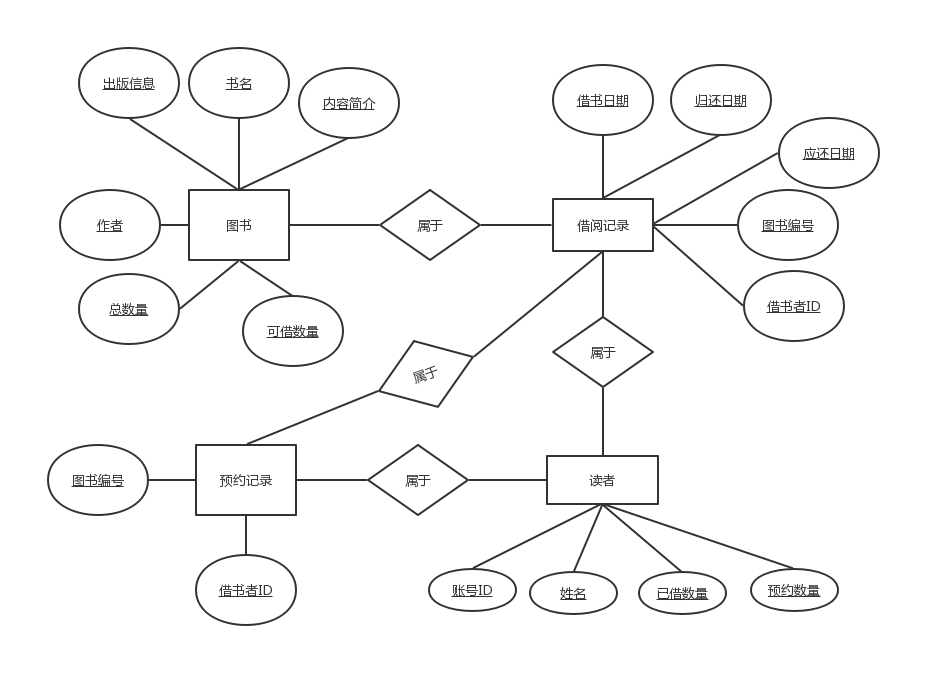
\includegraphics[width=0.7\textwidth]{./Chapters/images/ER.png} %插入图片,[]中设置图片大小,{}中是图片文件名
%     \caption{E-R图} %最终文档中希望显示的图片标题
%     \label{E-R图} %用于文内引用的标签   
% \end{figure}
\section{接口设计}
web客户端层的网络请求基于axios第三方api自定义,基础配置为:允许跨域;baseURL为'http://localhost:2222/apihttp://localhost:2222/api/';超时时间设置为10000毫秒;返回响应数据类型为json; 返回响应数据为UTF-8。

\textbf{获取图书列表}

url: 'api/book/list'

method: 'GET'

\begin{tabular}{lllll|}
    \hline
    Request URL参数& 类型& 是否必填& 默认值 & 备注\\
    pageNo & number & 是& 1& 页码\\
    pageSize & number & 是& 20& 页数\\
    keyword& string& 否& -& 关键词\\
    \hline
\end{tabular}

注:除了params对象外,还可传入自定义请求头,可包含登录token,CSRF校验token等信息。

\begin{tabular}{lllll}
    \hline
    Response data对象& 类型& 是否非空& 默认值 & 备注\\
    
    bookNo & number & 是& 1& 页码\\
    
    name & string& 是& 20& 页数\\
    
    author& string& 是& -& 作者\\
   
    press& string& 否& -& 出版社\\
    
    count& number& 是& -& 可借数量\\
    totalCount& number& 是& -& 馆藏总数量\\
    publishInfo& string& 否& -& 出版信息\\
    description& string& 是& -& 简介\\
    \hline
\end{tabular}

\textbf{提交借书请求:}

url: '/api/book/borrow';

method: 'POST';

\begin{tabular}{lllll}
    \hline
    Request body对象& 类型& 是否必填& 默认值 & 备注\\
    bookNo & number& 是& -& 图书编号\\
    userNo & number& 是& -& 读者编号\\
    createdTime& date& 否& Date.now()& 借书日期\\
    \hline
\end{tabular}

请求成功,response code返回200。

\textbf{获取预约列表:}

url: '/api/book/list/borrow';

method: 'GET'

\begin{tabular}{lllll}
    \hline
    Request URL参数& 类型& 是否必填& 默认值 & 备注\\
    
    pageNo & number & 是& 1& 页码\\
    
    pageSize & number & 是& 20& 页数\\
    \hline
\end{tabular}

\begin{tabular}{lllll}
    \hline
    Response data对象& 类型& 是否非空& 默认值 & 备注\\
    
    bookNo & number & 是& 1& 图书编号\\
    
    bookName & number& 是& 20& 图书名称\\
    
    expressNo& string& 是& -& 物流单号\\
    \hline
\end{tabular}

\textbf{获取个人信息:}

url: '/api/user/info';

method: 'GET'

\begin{tabular}{|l|l|l|l|l|}
    \hline
    Request URL参数& 类型& 是否必填& 默认值 & 备注\\
    \hline
    id & number & 是& -& 读者ID\\
    \hline
    name & number & 是& -& 读者姓名\\
    \hline
    address & string[] & 否& -& 收货地址\\
    \hline
\end{tabular}

如果上述请求成功,返回response的code为200,如果请求失败,返回下列code之一:

404:请求未找到

500:服务器内部错误

502:访问服务器被拒绝,响应无效

10002:用户鉴权失败

10005:字段类型错误

10012:其他原因,借书失败

\section{界面及交互设计}
\subsection{登录模块}
登录界面中输入借书账号和密码,验证通过则进入主界面,对于验证失败的情况:账号不存在,弹出toast提示"账号不存在,请前往图书馆申请注册借书卡,凭借书卡账号密码登录";账号密码填写错误,系统弹出提示"账号或密码填写错误"。用户点击下方注册按钮,则弹出modal提示"请前往图书馆注册借书卡,凭借借书卡账号密码登录"。
\begin{table}[ht]
    \centering
    \begin{tabular*}{\textwidth}{p{0.3\textwidth}p{0.7\textwidth}}
        \hline
        用户行为  & 系统显示 \\
        \hline
        进入登录界面 & 显示登录界面 \\
        输入账号密码 & 输入框显示用户刚刚输入的内容 \\
        点击登录按钮,登录失败 & toast显示提示文案:"账号不存在"或"账号或密码输入有误"\\
        点击登录按钮,登录成功 & toast显示"登录成功",显示加载条,跳转到主界面 \\
        \hline
    \end{tabular*}
    \begin{tabular*}{\textwidth}{p{0.3\textwidth}p{0.7\textwidth}}
        \hline
        窗口/对话框  & GUI组件 \\
        \hline
        登录界面 & 登录图标,登录表单:账号输入框,密码输入框,登录按钮 \\
        \hline
    \end{tabular*}
\end{table}
\subsection{主界面}
% \begin{figure}[H]
%     \centering
%     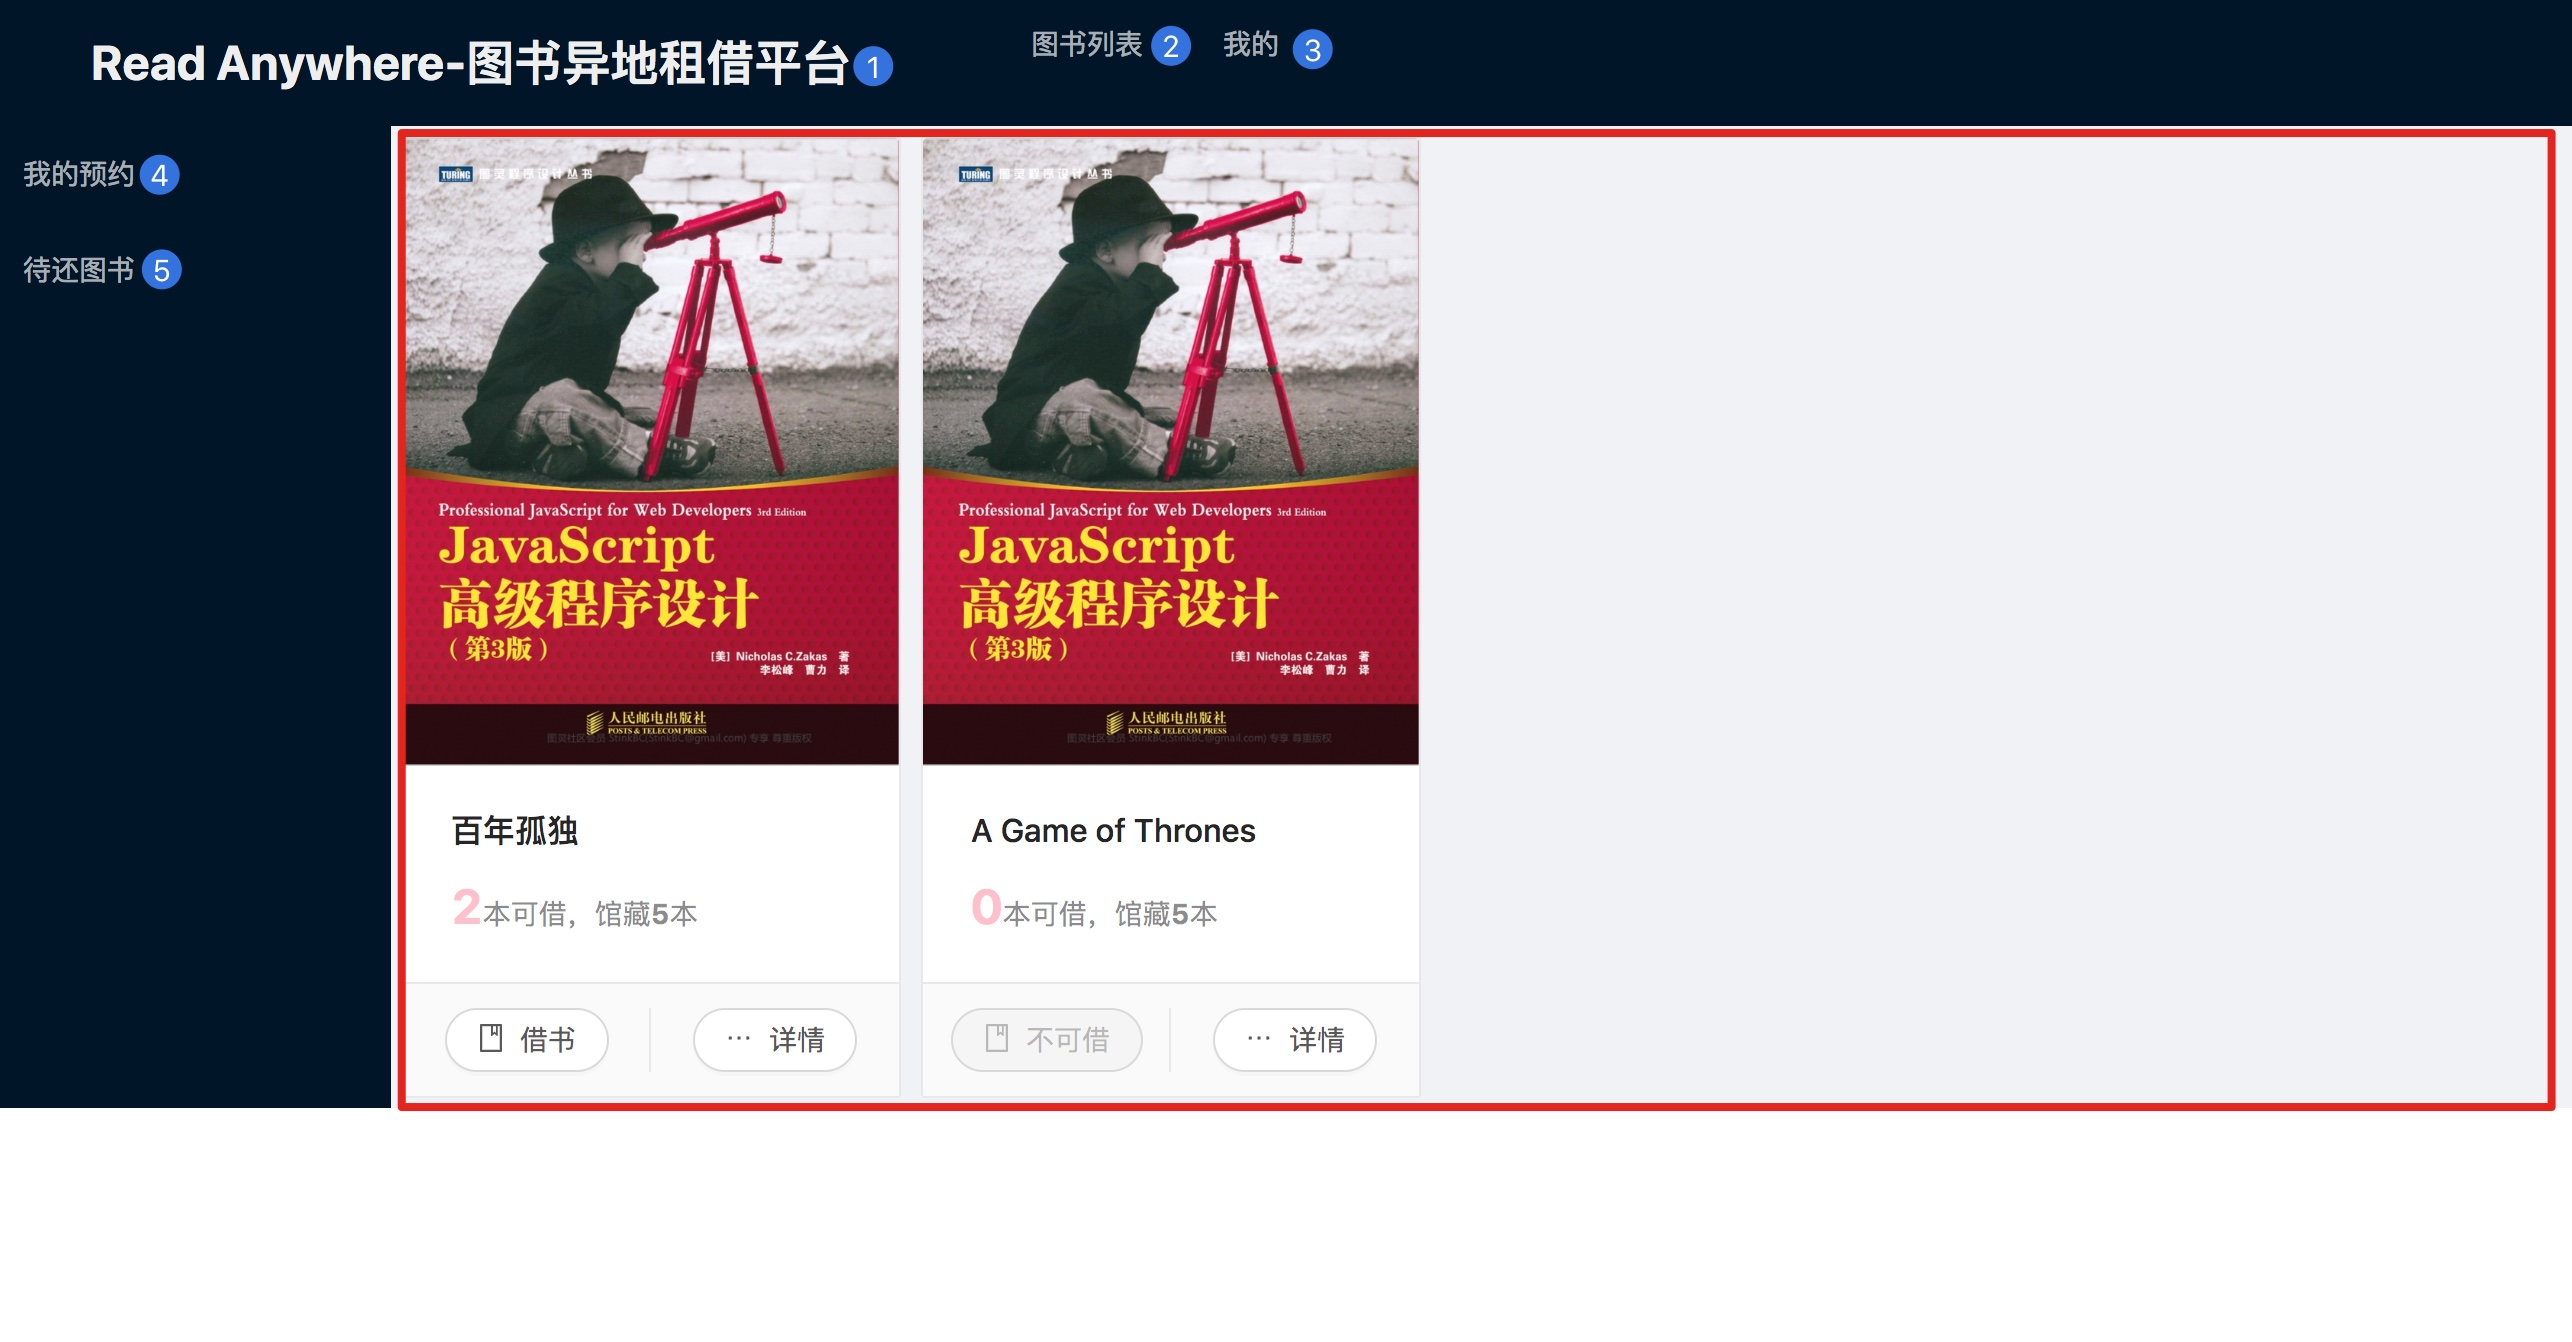
\includegraphics[width=\textwidth]{./Chapters/images/mainUI.png} %插入图片,[]中设置图片大小,{}中是图片文件名
%     \caption{界面设计-主界面} %最终文档中希望显示的图片标题
%     \label{界面设计-主界面} %用于文内引用的标签   
% \end{figure}
% 上图红色方框框住的部分为内容区,图中序号标注参考如下:
% \begin{enumerate}
%     \item 显示平台名称,字体格式为H1
%     \item 内容区默认显示的内容与点击“图书列表”导航按钮的内容一致,显示图书列表,每个列表项包含图书的封面、书名、馆藏数量、可借数量、简介等信息,馆藏数量大于0时,借书按钮可点击,否则不可点击。点击详情按钮,按钮上方弹出气泡,显示书籍简介信息
%     \item 点击“我的”导航按钮,内容区显示“我的”模块的信息
%     \item 点击“我的预约”菜单项,内容区显示预约列表
%     \item 点击“待还图书”菜单项,内容区显示待还图书列表
% \end{enumerate}
% 主界面的主框架包含上方导航栏、左侧菜单栏和底部信息栏。剩余的中部和右侧为内容区。内容区作为容器,根据导航栏或菜单栏的具体项显示对应数据。导航栏有"书籍列表"和"我的"两个Tab,页面的内容区默认显示"书籍列表"Tab下的内容。点击导航栏的"我的"Tab,内容区显示个人信息。进入主界面时会有网络请求,请求第一页的列表数据。
登录成功后系统会跳转到主界面,进入主界面时浏览器会发起网络请求,请求书籍列表数据。在网络请求成功之前界面一直显示Loading动画,数据请求成功后动画消失:
\begin{table}[ht]
    \centering
    \begin{tabular*}{\textwidth}{p{0.3\textwidth}p{0.7\textwidth}}
        \hline
        用户行为 & 系统显示\\
        \hline
        进入主界面 & 进入主界面时内容区显示加载圈,加载成功之后,内容区默认显示图书列表模块数据\\
        点击“图片列表”导航按钮 & 内容区显示图片列表信息 \\
        点击“我的”导航按钮 & 内容区显示“我的”模块的信息 \\
        点击“我的预约” & 内容区显示“预约列表”信息 \\
        点击“待还图书” & 内容区显示“待还列表”信息 \\
        点击“退出”按钮 & 退出系统,跳转至登录界面 \\
        \hline
    \end{tabular*}
    \begin{tabular*}{\textwidth}{p{0.3\textwidth}p{0.7\textwidth}}
        \hline
        窗口/对话框  & GUI组件 \\
        \hline
        导航栏 & 平台名称;“图书列表”按钮;“我的”按钮,用户姓名,退出按钮\\
        菜单栏 & “我的预约”菜单项;“待还图书”菜单项 \\
        内容区 & 根据用户点击的导航按钮或菜单项,显示对应模块的内容,默认显示图书列表模块的内容 \\
        \hline
    \end{tabular*}
\end{table}

用户点击导航栏或菜单项时,系统会对应加载数据,显示到内容区,如加载图书列表数据时:
\begin{enumerate}
    \item 请求成功且有数据,则将数据传入列表,展示到页面。书籍列表包含包含若干个卡片,每个卡片展示单本书籍的封面、条码号、作者、书名、简介、馆藏数量、可借数量,如果可借数量大于一本,则借书按钮是可点击的,否则按钮置灰,不可点击。
    \item 请求成功,但无数据,内容区展示"暂无数据"样式。
    \item 请求失败,弹出toast提示"请求失败,请重试",内容区展示"暂无数据"样式。
\end{enumerate}
用户点击导航栏的其他Tab,会发送网络请求请求对应数据,与上述"请求书籍列表"的逻辑流程类似。同时列表为分页懒加载,每页的数量为20条,用户点击对应页码按钮,请求和展示对应页码的数据。布局为弹性布局,根据窗口大小实现比例自适应。
\subsection{“图片列表”模块}
“图片列表”模块,显示书籍的信息,提供预约借书按钮和取消预约按钮,取消预约操作也可在预约列表中进行。
\begin{table}[ht]
    \centering
    \begin{tabular*}{\textwidth}{p{0.3\textwidth}p{0.7\textwidth}}
        \hline
        用户行为 & 系统显示\\
        \hline
        书籍可借数量大于1时,点击“借书”按钮 & 弹出二次确认框,确认后系统显示加载圈,请求结束后加载圈消失 \\
        书籍可借数量为0,点击“借书”按钮 & 按钮不可点击 \\
        点击“取消预约”按钮& 弹出二次确认框,确认后系统显示加载圈,请求结束后加载圈消失 \\
        点击“详情”按钮 & “详情”按钮上方显示气泡,气泡中显示书籍简介信息,再次点击或点击其他按钮,气泡消失 \\
        \hline
    \end{tabular*}
    \begin{tabular*}{\textwidth}{p{0.3\textwidth}p{0.7\textwidth}}
        \hline
        窗口/对话框  & GUI组件 \\
        \hline
        图书列表项 & 书籍封面;书名;可借数量;馆藏数量;预约按钮;详情按钮\\
        点击预约按钮后弹出的确认框 & 文案为:“确认预约本书?”,下方有确认按钮和取消按钮 \\
        书籍可借数量为0状态下的“借书”按钮 & 按钮置灰,不可点击\\
        点击详情按钮弹出的气泡 & 气泡在详情按钮正上方显示,高度不超过200px \\
        \hline
    \end{tabular*}
\end{table}
\newpage
\subsection{"我的"模块}
“我的”模块中,显示读者个人信息、收货地址,同时提供跳转至预约列表、待还列表的按钮。
\begin{table}[ht]
    \centering
    \begin{tabular*}{\textwidth}{p{0.3\textwidth}p{0.7\textwidth}}
        \hline
        用户行为 & 系统显示\\
        \hline
        点击“我的预约”列表项 & 跳转至预约列表,内容区显示预约列表数据\\
        点击“待还图书”列表项 & 跳转至待还列表,内容区显示待还图书数据 \\
        点击“物流地址”列表项& 列表项下方展开显示物流信息 \\
        \hline
    \end{tabular*}
    \begin{tabular*}{\textwidth}{p{0.3\textwidth}p{0.7\textwidth}}
        \hline
        窗口/对话框  & GUI组件 \\
        \hline
        “我的”界面 & 用户姓名;账号ID;“待还图书”列表项;“我的预约”列表项;“物流地址”列表项\\
        “物流地址”列表项 & 该列表项为一个折叠面板,点击展开,显示物流信息列表,包含列表项、新增地址按钮,每个列表项包含:联系人手机号;详细地址,编辑按钮,删除按钮;再次点击折叠面板收起 \\
        \hline
    \end{tabular*}
\end{table}
\newpage
\subsection{“我的预约”模块}
\begin{table}[ht]
    \centering
    \begin{tabular*}{\textwidth}{p{0.3\textwidth}p{0.7\textwidth}}
        \hline
        用户行为 & 系统显示\\
        \hline
        点击“取消预约” & 弹出二次确认框,确认框文案为:“确认取消预约?”\\
        \hline
    \end{tabular*}
    \begin{tabular*}{\textwidth}{p{0.3\textwidth}p{0.7\textwidth}}
        \hline
        窗口/对话框  & GUI组件 \\
        \hline
        预约列表项 & 书籍名称;预约日期;取消预约按钮\\
        预约列表 & 展示20条列表项,列表下方有分页按钮\\
        \hline
    \end{tabular*}
\end{table}
点击二次确认框之后,系统会显示加载圈,请求结束后加载圈消失,不同请求结果对应样式:
\begin{enumerate}
   \item 请求成功,弹出toast"请求成功",该列表项被删除,不再出现在预约列表中。
   \item 请求失败,弹出toast"请求失败,请重试",列表维持原样无变化。 
\end{enumerate}
\subsection{“待还图书”模块}
\begin{table}[ht]
    \centering
    \begin{tabular*}{\textwidth}{p{0.3\textwidth}p{0.7\textwidth}}
        \hline
        用户行为 & 系统显示\\
        \hline
        点击“我要还书” & 弹出表单框,填写物流信息\\
        点击表单框中的确认按钮 & 表单校验成功之后,显示加载圈,请求结束后加载圈消失,表单框消失\\
        点击表单框中的取消按钮 & 表单框消失。\\
        \hline
    \end{tabular*}
    \begin{tabular*}{\textwidth}{p{0.3\textwidth}p{0.7\textwidth}}
        \hline
        窗口/对话框  & GUI组件 \\
        \hline
        待还列表项(未填写过还书物流) & 书籍名称;借书日期;预约的物流单号;我要还书按钮\\
        待还列表项(已填写还书物流) & 书籍名称;借书日期;预约的物流单号;还书的物流单号;还书日期;修改物流按钮\\
        点击还书后弹出的表单框 & 表单中包含物流公司输入框;物流编号输入框;确认按钮;取消按钮。输入框内容均为空 \\
        点击修改物流后弹出的表单框 & 表单中包含物流公司输入框;物流编号输入框;确认按钮;取消按钮。输入框内容为上次填写的物流公司名和单号\\
        \hline
    \end{tabular*}
\end{table}
% 点击待还列表,路由跳转至对应页面,内容区展示一个懒加载的分页列表,页数20,每个列表项显示待还书籍的书名、条码号和"我要还书"按钮。点击"我要还书书",页面弹出modal框,在modal框的表单内填入物流信息,点击确认,发送对应网络请求。列表栏会显示对应物流单号和快递公司名称,右侧有一个编辑按钮,点击可修改物流信息。有物流单号时,不显示"我要换书"按钮。

% 收货地址栏中,包含收货地址信息,可新增、编辑、删除单条收货信息。每条收货地址信息的姓名、联系人号码、街道地址为必填。

% 点击退出按钮,弹出二次确认框,用户点击确认后,跳转至登录界面。






